%************************************************
\chapter{Introduction}\label{ch:introduction}
%************************************************

The \ac{IoT} is a term with a wide range of interpretations \citep{Atzori20102787}, breafly, we can think of it as a set of devices, mainly resource constrained, that are interconnected between them in order to achieve a goal. For example, a network of lampposts with proximity sensors that talk to each other so they light up part of the street when a passerby walks by, but save energy when not; greenhouses with automated irrigation to balance costs and quality vegetables; or cars exchanging traffic data to reduce city pollution from traffic jams or avoid accidents.

Many of this objectives require the use of a great amount of data, and thanks to organizations like \href{https://wikileaks.org/}{WikiLeaks}, people are aware of the implications of their data on the Internet, demanding more security and privacy for it. This includes not only the data shared with others, where one must trust they will keep it safe, but it's also the data collected about us and that we don't have direct control over it. The attack Sony suffered in 2011 to PSN \citep{PSN2011} is an example of the trust people had in Sony to store their billing information, and because the security of that information depended on both them and Sony, people found themselves compromised unable to do anything about it. 

With the proliferation of IoT devices gathering as much information as they can with their sensors, the amount of data gathered about anyone can be immense. And IoT has proved to not address neither security nor privacy, with recent events like the Mirai botnet DDoS attack on October 2016, considered the biggest DDoS in history \citep{jeyanthi:2017}, or the multiple vulnerabilities affecting house devices, like baby monitors \citep{rapid7babycam}.


To address this problem of privacy in the Internet, a recent approach is the concept of \textit{strong anonymity}, that conceals our personal details while letting us continue to operate online as a clearly defined individuals \citep{stronganonymity}. To achieve it, we must address a way to perform authentication and authorization in the most privacy-friendly approach. Attribute-based credentials and \textit{selective disclosure} allow to control what information we reveal, under a trusted environment.

Intuitively, an attribute-based credential can be thought of as a digital signature by the Issuer on a list of attribute-value pairs, e.g. the list \texttt{\justify(fname=Alice, lname=Anderson, bdate=1977-05-10, nation=DE)} \citep{introCredIBM}.
The most straightforward way for the User to convince a Verifier of her list of attributes would be to simply transmit her credential to the Verifier.
With anonymous credentials, the User never transmits the credential itself, but rather uses it to convince the Verifier that her attributes satisfy certain properties – without leaking anything about the credential other than the shown properties. This has the obvious advantage that the Verifier can no longer reuse the credential to impersonate \texttt{Alice}. Another advantage is that anonymous credentials allow the User to reveal a selected subset of her attributes.
Stronger even, apart from showing the exact value of an attribute, the User can even convince the
Verifier that some complex predicate over the attributes holds, e.g. that her birth date was more than 18 years ago, without revealing the real date.


With usual symmetric and asymmetric cryptography it seems impossible to create such credentials, without an explosion of signatures over every possible combination. Thats why current solutions rely on  \acp{ZKP}
\marginpar{To read more about ZKPs, refer to my Mathematics thesis \citep{tfgmates}.}
, cryptographic methods that allow to proof knowledge of some data without disclosing it.

To understand how ZKPs work, in 1990 Guillou, Quisquater and Berson published in \textit{How to Explain Zero-Knowledge Protocols to Your Children} \citep{ZKPcave:story} a story about how Ali Baba proved that he knew the magic words to open the cave, but without revealing those words to anyone. Here we present a brief version highlighting the properties of ZKPs.

\hfil

\begin{quote}
	Imagine a cave, where the path forks in two passages, and at the end of each one, they join again, with the shape of a ring. In the point the paths meet, there is a magic door, that only opens when someones pronounces the magic work.
	
	\textbf{P}eggy knows the secret word and wants to \textbf{p}rove it to her friend, \textbf{V}ictor, but without revealing it.
	\marginpar{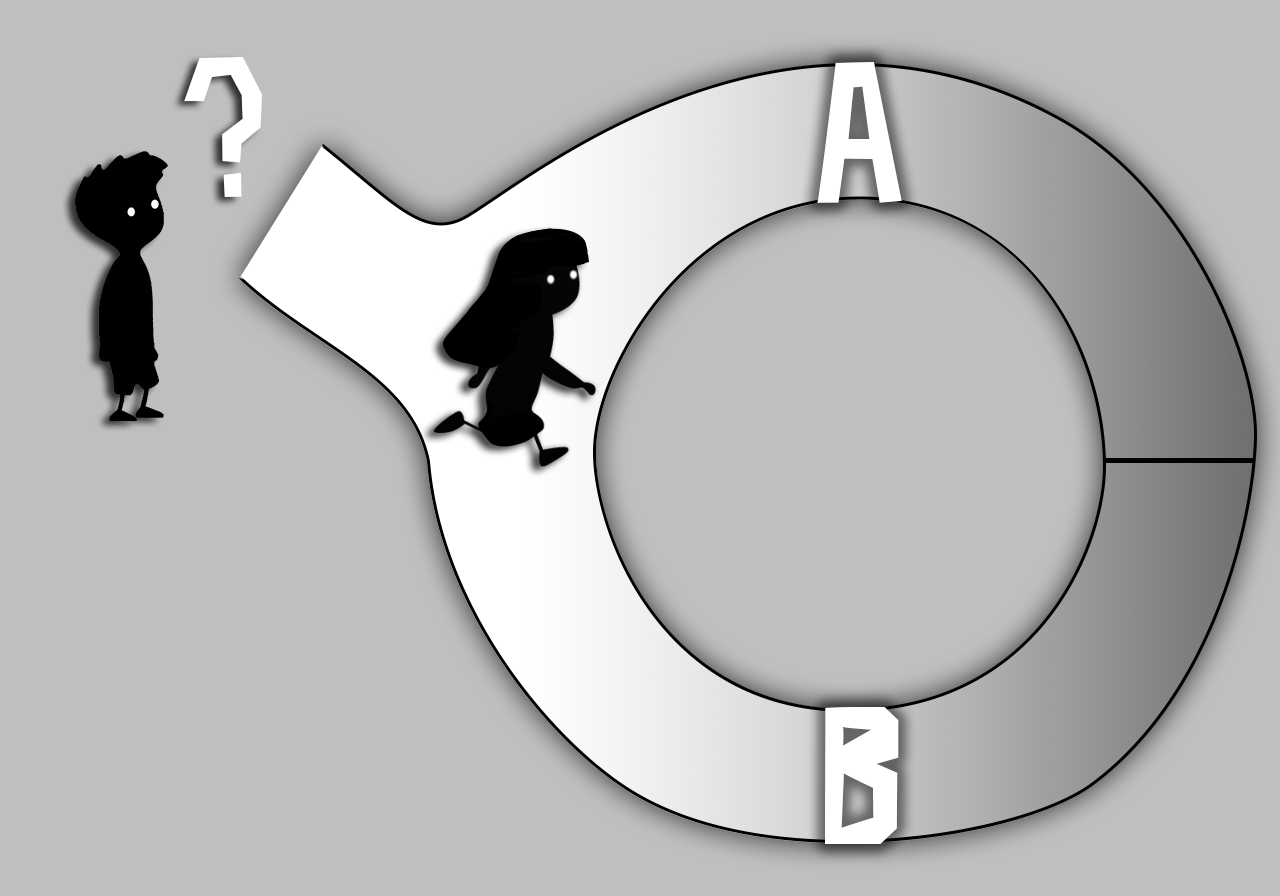
\includegraphics[width=1.\linewidth]{gfx/graficoJL_ZKP_1}\\The cave \citep{ZKPcave:fig}
		. Peggy takes randomly A or B. Victor awaits outside.}
	Peggy and Victor meet at the entrance of the cave, then Victor awaits while Peggy goes inside the cave, taking one of the passages, that we will name A and B. Victor can't see which way Peggy went. 
	
	When Peggy arrives at the door, \textbf{V}ictor enters the cave, and when he arrive to the fork, stops and yells which path, A or B, he wants Peggy to come back, to \textbf{v}erify she knows how to open the door.
	
	If Peggy actually knows the secret, she always can take the requested path, opening the magic door if needed.
	\marginpar{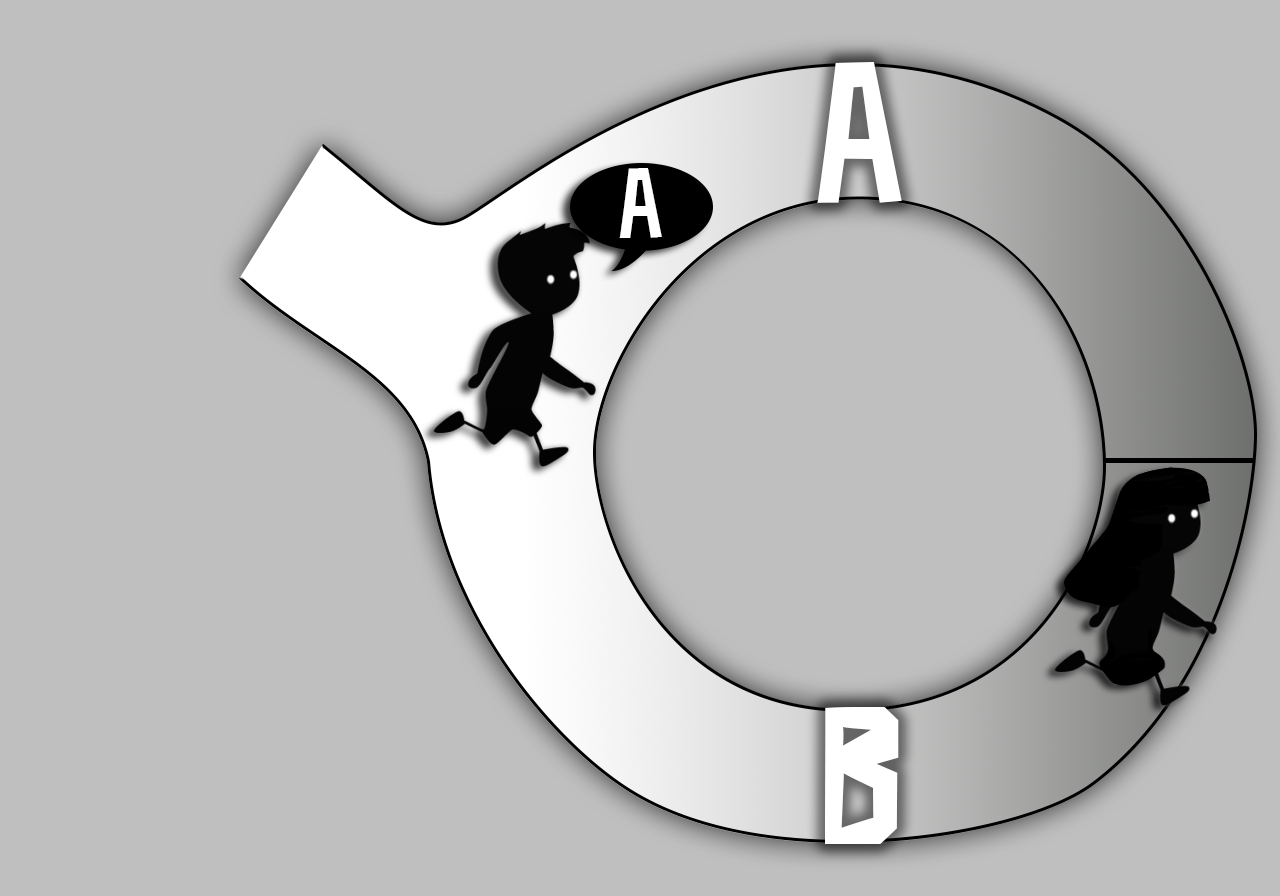
\includegraphics[width=1.\linewidth]{gfx/graficoJL_ZKP_2}\\The cave. Victor chooses randomly the returning path for Peggy.}
	But if Peggy doesn't know the magic word, she had a chance of $50\%$ to guess correctly what passage Victor was going to ask. That means she had a chance to fool Victor.
	
	Victor then asks to repeat the experiment. With $20$ repetitions, the chances Peggy fools Victor in all of them is only  $2^{-20}$,
	\marginpar{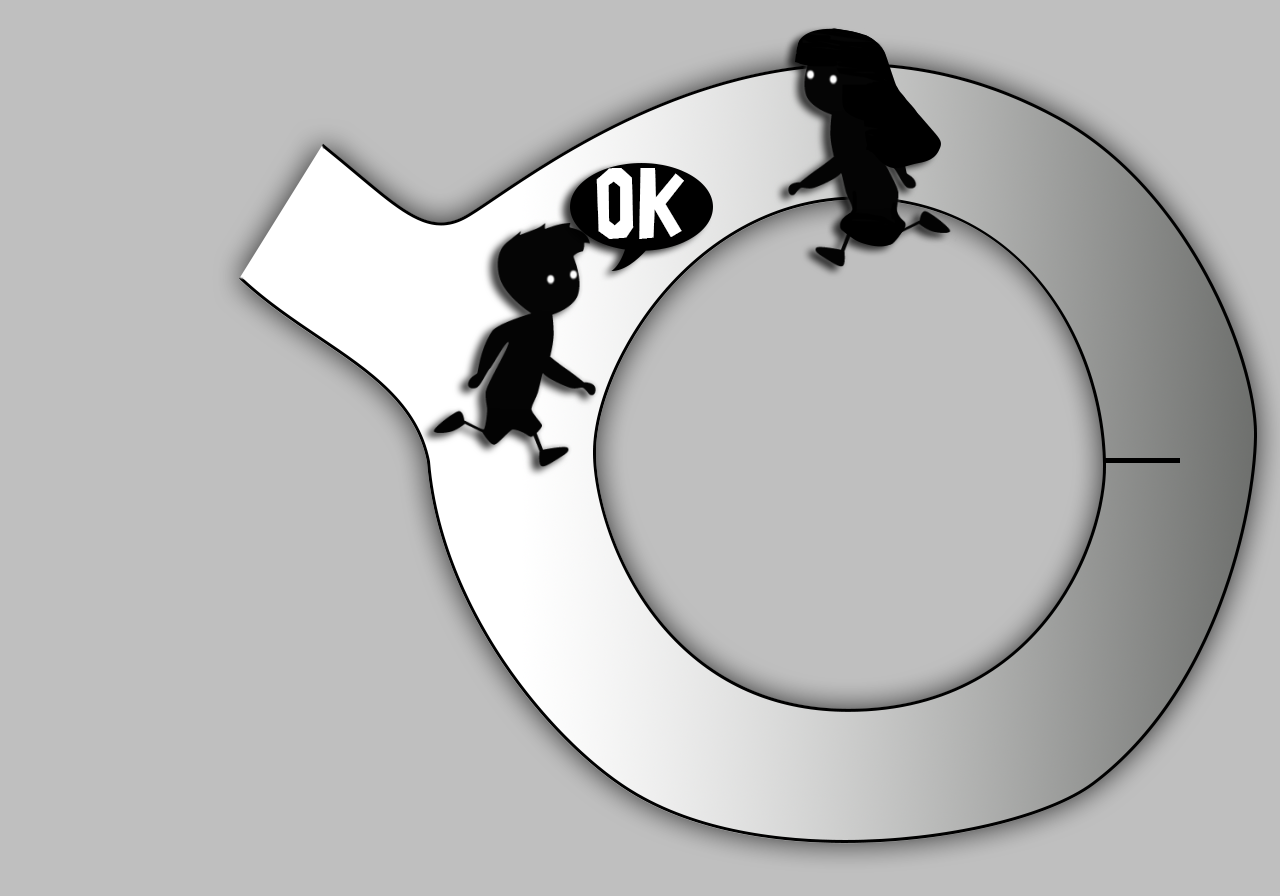
\includegraphics[width=1.\linewidth]{gfx/graficoJL_ZKP_3}\\The cave. Peggy returns by the requested path.}
	
	\textbf{E}ve, curious about what Victor and Peggy were doing in the cave, \textbf{e}avesdrops Victor during the process. The problem is that Eve doesn't know if Peggy and Victor agreed on what paths to choose, because they wanted to prank her for being busybody. Only Victor is confident he is choosing the returning passage randomly.
	
	Later, Victor is convinced that the door can be opened and Peggy knows the word, but he can't prove it to Eve because he can't open the door. 
\end{quote}





Based on ZKP properties, IBM has developed the Identity Mixer\footnote{Identity Mixer - \url{https://www.research.ibm.com/labs/zurich/idemix/}}, Idemix for short, protocol suite for privacy-preserving authentication and transfer of certified attributes. It allows user authentication without divulging any personal data. Users have a personal certificate with multiple attributes, but they can choose how many to disclose, or only give a proof of them, like being older than 18 years-old, living in a country without revealing the city, etc. Thus, no personal data is collected that needs to be protected, managed, and treated.

\begin{center}
	\textit{``If your personal data is never collected, it cannot be stolen.''}
\end{center}

The goal of this project is to integrate Idemix with the IoT. It will be done using the ABC4Trust's \ac{P2ABCE}, a framework that defines a common architecture, policy language and data artifacts for an attribute based ecosystem, cryptographically based on either IBM's Idemix or Microsoft's U-Prove \citep{p2abcurl}. This gives us a standardized language to exchange Idemix's messages between IoT devices and any other P2ABCE actor.

\hfil


\section{Outline of this thesis}

This document is structured as follows: In \autoref{ch:stateoftheart} we show a state of the art analysis through the history of Idemix and related works, analysing what is of the most interest for the IoT perspective; then, in \autoref{ch:objectives} we outline the project's objectives and analyse in depth the existing solutions that we are going to deal with; in \autoref{ch:design} we describe the formal design of the IoT and Idemix solution, and describe the PoC implementation developed; after an implementation, it is a must to validate it, as showed during the performance tests in \autoref{ch:validation}; finally, our conclusions and lines for future work are described in \autoref{ch:conclusions}.

